\documentclass[a4paper,11pt,oneside,%twoside to print on the back of pages
headsepline,												% Linie für Kopfzeile
footsepline,												% Linie für Fußzeile
bibtotocnumbered									% numb point literaturverz in inhaltsverz => bibliography=tot ocnumbered
]{scrreprt}
%----------------------------------------------------------------------------------------------------------------------------------------------
% STANDART LIBS
\usepackage[T1]{fontenc}
\usepackage[utf8]{inputenc}
\usepackage[ngerman]{babel}    % Deutsche Sprache in automatisch generiertem

% DRUCKBEREICH: \areaset[BCOR]{textwidth}{textheight} %TODO understand
% BCOR ist "Binding Correction", also wieviel Innenrand verloren geht
% A4 hat 297mm x 210mm
% wenn keine Marginalien, dann ist Breite 15cm vielleicht besser
\areaset[1.5cm]{14cm}{25cm} 
%% Die folgende Zeile sorgt dafür, daß die Fußnoten eingerückt werden,
%% und zwar um 2em (class scrbook).
\deffootnote{2em}{2em}{\textsuperscript{\normalfont\thefootnotemark} }

%----------------------------------------------------------------------------------------------------------------------------------------------
% ADDITIONAL LIBS

\usepackage{grffile} %remove file names of images

% Wrapping text around figures
\usepackage{wrapfig}  %
% containers for things that cannot be broken over a page -> example table, figure
\usepackage{float}
% provides many ways to customise the captions in floating environments
\usepackage{caption} % http://www.ctex.org/documents/packages/float/caption.pdf
% same for subfigues
\usepackage{subcaption} % hint include subpicture

%% Unterstützung für Graphiken und Farben
\usepackage[pdftex]{graphicx}
%\usepackage[pdftex]{color}
%\definecolor{DSblue}{rgb}{0,0,0.9}   % example defining a color



% INDEX/GLOSSARY %TODO
%Defines commands for use with MakeIndex
%\usepackage{makeidx} % -> en.wikibooks.org/wiki/LaTeX/Indexing pctex.com/files/managed/3/3a/makeindx.pdf
%\usepackage[xindy,toc]{glossaries}
\usepackage{acronym} %Abkürzungsverzeichniss

%BIBTEX
%used by biblatex for qutes
\usepackage[babel,german=quotes]{csquotes} % load after inputenc
% cite package -> 1. pdflatex xx.tex 2. biber xx 3. pdflatex xx.tex
\usepackage[style=reading,backend=biber]{biblatex} %TODO check diff cite styles
% loads the bib file
\addbibresource{bachelorBib.bib}


% cross referencing and hyperrefs
\usepackage[                % FIXME explain
   pdftex,                  % Ausgabe-Medium: PDF
   colorlinks=true,         % farbige Links in der Bildschirm-Version?
   pdfstartview=Fit,       % wie soll Acrobat starten?
   linkcolor=black,         % Farbe für Querverweise
   citecolor=black,         % Farbe für Zitierungen
   urlcolor=black,          % Farbe für Links
   bookmarks=true
   ]{hyperref}
% non clickable URL   		
\usepackage{url} %TODO remove if hyperref is better

% TODONOTES -> http://tex.stackexchange.com/questions/9796/how-to-add-todo-notes
\usepackage{lipsum}                     % Dummytext
\usepackage{xargs}                      % Use more than one optional parameter in a new commands
\usepackage[pdftex,dvipsnames]{xcolor}  % Coloured text etc.
% -> www.tex.ac.uk/ctan/macros/latex/contrib/todonotes/todonotes.pdf
\usepackage[colorinlistoftodos,prependcaption,textsize=tiny]{todonotes}
\newcommandx{\unsure}[2][1=]{\todo[linecolor=red,backgroundcolor=red!25,bordercolor=red,#1]{#2}}
\newcommandx{\change}[2][1=]{\todo[linecolor=blue,backgroundcolor=blue!25,bordercolor=blue,#1]{#2}}
\newcommandx{\info}[2][1=]{\todo[linecolor=OliveGreen,backgroundcolor=OliveGreen!25,bordercolor=OliveGreen,#1]{#2}}
\newcommandx{\improvement}[2][1=]{\todo[linecolor=Plum,backgroundcolor=Plum!25,bordercolor=Plum,#1]{#2}}
\newcommandx{\thiswillnotshow}[2][1=]{\todo[disable,#1]{#2}}

% Print graphics
% tikz print graphs: http://www.texample.net/tikz/examples/
% bytefield – Create illustrations for network protocol specifications

% source code include
\usepackage{listings} % -> %TODO use minted
\usepackage{minted}

\makeatletter
\newcommand*{\rom}[1]{\expandafter\@slowromancap\romannumeral #1@}
\makeatother

%----------------------------------------------------------------------------------------------------------------------------------------------
% ADDITIONAL LIBS TO CHECK

%linien in Tabellen
\usepackage{booktabs}
\usepackage{anysize}
\usepackage[onehalfspacing]{setspace}


% math for matrix and $$
%\usepackage{amsmath}
%\usepackage{amssymb}

%\usepackage{lmodern}

%\usepackage{multido}    % FIXME ???????????
%\usepackage{everysel}   % FIXME ???????????
 
%% besserer Flattersatz: \RaggedRight
\usepackage{ragged2e}

% from exposee
\usepackage{latexsym}         % Fuer recht seltene Zeichen

\usepackage[a4paper,lmargin={2.5cm},rmargin={2.5cm},tmargin={3cm},bmargin={2.5cm}]{geometry}
\usepackage{enumerate}

\newcommand{\HRule}{\rule{\linewidth}{0.5mm}}

\pdfinfo{
	/Title		(Synchronisation von Binärbaum-indexierten, verteilten InMemory-NoSQL-Datenbanken)
	/Subject		(Bachelorarbeit)
	/Author		(Paul Kitt)
}
%----------------------------------------------------------------------------------------------------------------------------------------------
\pagenumbering{roman}
\begin{document}

%TODO set 1,5 zeilenabstand , verdana, schriftgroesse 10
%TODO check bewilligten title 


\begin{titlepage}
	\begin{center}
		\begin{figure}[!htb]
			\minipage{0.5\textwidth}
				\begin{center}
			  		
\includegraphics[width=0.5\textwidth]{bilder/htwLogo.jpeg}
				\end{center}
			\endminipage\hfill
		 	\minipage{0.5\textwidth}
				\begin{center}
			 		
\includegraphics[width=0.5\textwidth]{bilder/Spinning_O_Wheel-200.png}
				\end{center}	
			\endminipage
		\end{figure}
	
		 \vfill
		 \HRule \\[0.4cm]
	    {\bfseries\Large
	        \begin{LARGE}
	        Synchronisation von Binärbaum-indexierten, verteilten
			InMemory-NoSQL-Datenbanken\\
	        \end{LARGE} 
	    }    
		\HRule \\[1.5cm]
			\begin{minipage}{1.0\textwidth}
				\begin{flushleft}
				\Large	Abschlussarbeit
				\end{flushleft}
			\end{minipage}
			\vfill
			\begin{minipage}{1.0\textwidth}
				\begin{flushleft}
					\Large zur Erlangung des akademischen Grades\\
					\Large Bachelor of Science (B.Sc.)
				\end{flushleft}
			\end{minipage}
			\vfill
			\begin{minipage}{1.0\textwidth}
				\begin{flushleft}
					\Large an der
				\end{flushleft}
			\end{minipage}
			\vfill
			\begin{minipage}{1.0\textwidth}
				\begin{flushleft}
					\Large Hochschule für Technik und Wirtschaft Berlin\\
					\Large Fachbereich Wirtschaftswissenschaften \rom{2}\\
					\Large Studiengang Angewandte Informatik\\
				\end{flushleft}
			\end{minipage}
			\vfill
			\begin{minipage}{1.0\textwidth}
				\begin{flushleft}
					\Large 1. Prüfer: Prof. Dr.-Ing. Hendrik Gärtner\\
					\Large 2. Prüfer: Jens-Peter Haack\\ \todo[inline]{Titel Adademischer Grad}
				\end{flushleft}
			\end{minipage}
			\vfill
			\begin{minipage}{1.0\textwidth}
				\begin{flushleft}
					\Large Eingereicht von Paul Kitt
				\end{flushleft}
			\end{minipage}

		\vfill
		\begin{minipage}{1.0\textwidth}
			\begin{flushleft}
				{\Large \today}
			\end{flushleft}
		\end{minipage}
		\vfill

	\end{center}
\end{titlepage}
\tableofcontents
\newpage
%\todo[inline]{table of table}
%\todo[inline]{table of listings}
Abkürzungsverzeichniss:\\
\begin{acronym}[EB-Baum] % option laengest abk def einzuglänge
 	\acro{EB-Baum}{Elastische Binär Baum}
 	\acrodefplural{EB-Baum}[EB-Bäume]{Elastische Binär Bäume}
 	\acro{ID}{Identifikationsnummer}
\end{acronym}
\renewcommand\listoflistingscaption{Verzeichnis aller Codebeispiele}
\listoflistings

	%---------------------------------------------------------------------------------------------------------------------------------------------------	
\chapter{Einleitung}
\pagenumbering{arabic}
\todo[inline]{Hintergrund, größerer Rahmen, kurze Aufgabenstellung}
 		\begin{enumerate}[1.]
			\item  Problemstellung und Motivation
			\item Zielsetzung
			\item Rahmen und Aufbau der Arbeit
		\end{enumerate}
		
	Mögliche Punkte:
	-> Motivation
	-> Aufgabenbeschreibung
	-> Inhalt und Aufbau der Arbeit	
		
	%---------------------------------------------------------------------------------------------------------------------------------------------------	
\chapter{Grundlagen}
\todo[inline]{	theoretische Grundlagen, Beschreibung von Systemen(nur insoweit, als das diese Grundlagen und Beschreibungen unbedingt für das Verständnis erforderlich sind und nicht als bei studierten Informatikern vorausgesetzt werden kann)}

	\begin{enumerate}[1.]
			\item Grundlagen verwendeter Algorithmen
				\begin{enumerate}[1.]
					\item Binär Bäume
					\item Elastische Binär Bäume
				\end{enumerate}
			\item Definition von Begriffen
				\begin{enumerate}[1.]
					\item Verteilung
					\item Synchronisation
					\item NoSql -> CAP, ACID theoreme die meine db erfüllt 
				\end{enumerate}
			\item Grundlagen Datenbanken (Verteilung, Synchronisation)
				\begin{enumerate}[1.]
					\item MySql
					\item NoSql 
					\item Baumbasierter Indexe
				\end{enumerate}
	\end{enumerate}

\section{Elastische Binär Bäume}
\label{sec:ebTreeGrundlagen}
Bei den \enquote{Elastischen Binär Bäumen} handelt es sich um speziell optimierte Variante der \enquote{Binären Suchbäume}. Entwickelt wurden das Konzept von Willy Tarreau\autocite{Tarreau} im Rahmen einer Forschung zum Thema \enquote{Event-scheduling for user-space network applications} und eignen sich daher auch speziell für Betriebssystem Scheduler, bei welchen schnelles priorisieren nach Zeit oder Dringlichkeit wichtig ist. Daten die mit Binär- oder Ganzahlen, wie Integer oder Long, indexiert sind können in dieser wenig bekannten Datenstruktur sehr effizient verwaltet werden. Dabei ist der \enquote{\ac{EB-Baum}} sehr performant wenn es zu sehr vielen den, Baum verändernden, Operationen, wie: Einfügen, Ändern, Abfragen oder Löschen kommt.\unsure{wie richtig zitieren?}\\
Einfügeoperationen und das Abfragen von Blättern wird in O(log n) bewältigt. Löschen in O(1).\\

Als Ausgangskonzepte dienten bei seiner Entwicklung der \enquote{balanciertem Binär Baum}\unsure{mention red black tree} und des \enquote{Radix Baumes}. Da aber Operationen wie Löschen von Blättern bei einem \enquote{balanciertem Binär Baum} O(log n) kosten und der Baum aber gerade Operationen wie diese möglichst schnell bewältigen soll ein signifikanter Nachteil. Bei den \enquote{Radix Bäumen}, die sich laut dem Entwickler Willy Tarreau\autocite[Absatz Introduction]{Tarreau} im Bezug auf Geschwindigkeit sehr gut eigenen, wird aber im Betrieb das allocieren von Speicher und die damit verbundene \enquote{Garbage Collection} zum Perfomanceproblem.\\

Daher ist der \ac{EB-Baum} eine hybride Form aus beiden um diese Mängel aus zu gleichen. Es handelt sich nicht um einen balancierten Baum, was in besonderen Fällen zu einer schlechteren Leistung als die eines \enquote{balanciertem Binär Baum} führt\unsure{mention example}. Die Blätter sind im Baum von links nach rechts aufsteigend, nach einer Binär- oder Ganzahl(e.g. Integer, Long) sortiert.\\

Eine weitere Besonderheit des \ac{EB-Baum} ist dass seine maximale Höhe durch den Datentyp der Schlüssel bestimmt wird.
So kann beispielsweise ein Baum dessen Schlüssel Werte des Datentypes \enquote{Long} sind maximal 64 Ebenen besitzen da der Datentyp aus 64 Bit besteht. Schlüssel werden durch die Abfolge ihrer Binären Repräsentation adressiert. Der Schlüssel dient hierbei wie eine Art binäre Karte. Begonnen am höchsten gesetzten Bits des Schlüssels und wird der Baum Knoten für Knoten durch laufen und an den Knoten bei einer Null links, bei einer Eins rechts abgebogen bis dass Blatt oder falls dieses nicht vorhanden das am naheliegendste gefunden ist

\subsection{Besonderheiten des Baumes}
Durch die besondere Beschaffenheit des Baumes lassen sich viele Operationen sehr leicht umsetzen wie:
\begin{itemize}
	\item \textbf{Abfragen}
	\begin{itemize}
		\item das Abfragen des ersten und letzten Schlüssels
		\item erlangen des nächst kleineren oder größerem Schlüssel zu einem gegeben Schlüssel
		\item genaues Finden eine Schlüssels
		\item das Finden des ähnlichsten Schlüssels falls dieser nicht enthalten ist
		\item einfaches Abfragen von Bereichen durch ein Prefix
		\item erlangen des vorherigem oder nächstem unterschiedlichen Schlüssel zu einem gegeben Schlüssel
		\item mehrfach auftretende Schlüssel werden immer in ihrer eingefügten Reihenfolge zurück gegeben
	\end{itemize}
	\item \textbf{Einfügen}
	\begin{itemize}
		\item Einfügen mit Duplikaten: Falls ein Werte bereits existiert wird ein Duplikat angelegt
		\item Einfügen von nur einzigartigen Schlüsseln: Falls der Schlüssel vorhanden wird Existierende zurück gegeben
	\end{itemize}
\end{itemize}


\subsection{Aufbau des Baumes}
In dem originalem von Willy Tarreau verfassten Konzept\autocite[Absatz Definitions]{Tarreau} werden die Daten, die Baum hält, in \enquote{EB Knoten}
gespeichert. \enquote{EB Knoten} bestehen aus zwei Teilen:
\begin{itemize}
\item Knoten: verknüpft Blätter sowie anderen Knoten
\item Blatt: ist durch einen Schlüssel adressiert, hält Daten e.g. Referenz auf ein Datenobjekt
\end{itemize}


\begin{wrapfigure}{r}{0.6\textwidth}
  \begin{center}
    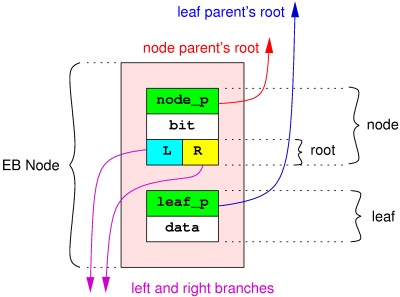
\includegraphics[width=.6\linewidth]{bilder/Ebnode.png}
  \end{center}
 \caption{EB-Knotenelement}
\end{wrapfigure}
Die Aufgabe eines Blattes ist sehr simpel. Es dient nur dazu eingefügte Daten durch einen Pointer zuhalten. Dabei ist es mit einem Schlüssel adressiert und besitzt eine Referenz auf seinen Elternknoten, sowie auf seinen EB-Ursprungsknoten\unsure{SPW fragen}.\\

Ein jedes Knotenelement besteht aus einer Referenz auf sein höher liegenden Elternknoten, dem Ebenenbit \unsure{Darf ich das Bild benutzen?} und zwei Referenzen auf seine Kinderknoten. \\ Das Ebenenbit ist eine Zahl und repräsentiert binär die niedrigste Bitposition des Schlüssels über dem alle Bits gleich sind. Alle unter dem Knoten liegenden Schlüssel haben sich somit bis zu diesem Bit die gleich Bitfolge. Der dritte Teil des Knotens ist die Wurzel die aus zwei Referenzen besteht zu entweder weiteren Knoten oder/sowie Blättern verweist. Da es sich um einen binären Baum handelt repräsentiert je Referenz das linke Bit 0 oder das rechte 1. Nur auf Ebene 0, mit dies repräsentierendem Ebenenbit, kann der Knoten zwei Blätter als Wurzel besitzen, da der Schlüssel sich nur um einen Wert an der letzten, nullten Bitstelle unterscheiden kann.\\
Auch wenn Knoten sich später verschieben können diese nie unterhalb des mit ihnen angefügtem Blattes oder in einen anderen Zweig des Baumes gelangen. Falls es erlaubt ist Duplikate einzufügen werden  Knoten mit negativen Ebenenbits versehen.\\

Eine weitere Besonderheit hier ist dass die Wurzelreferenzen nie unbelegt sind. Nur die Wurzel des Wurzelknoten des Baumes ist hier eine Ausnahme. Wenn seine zwei Wurzeln auf \enquote{null} referenziert ist der Baum leer. Sobald der Baum befüllt wird wächst dieser an seiner linken/\enquote{0-Wurzel}. Die rechte Wurzel referenziert immer auf \enquote{null}. Dadurch lässt sich der der Wurzelknoten einfach erkennen.
Sein Ebenenbit ist die höchste Ebene des Baumes und daher automatisch die binäre Länge des Schlüsseldatentyps, e.g. bei Schlüsseln des Datentyps Long ist das Ebenenbit 64.\\

\subsection{Einfügen von Daten}
Beim einfügen neuer Datensätze wird jeweils ein Blatt, das die Daten hält, sowie ein Knoten mit dem dass Blatt in Kombination eingefügt wird, eingefügt. Der einzige Fall in dem ein Blatt ohne Knoten angefügt wird ist wenn der Baum leer ist.

Beim Einfügen eines neuen Datensatzes wird ein gesamter \enquote{EB-Knoten} erstellt und an der richtigen Position eingefügt. Werden später weitere Werte gespeichert wird bei deren sortiertem einfügen der Baum umstrukturiert. Dies hat zur Folge dass Knoten und Blatt eines vorher übereinander liegenden \enquote{EB-Knoten} auseinander gezogen werden. Da sie aber noch durch gegenseitige Referenzen\unsure{logisch} verbunden bleiben wird der Baum als elastisch bezeichnet was zum Namen \enquote{\ac{EB-Baum}} führt.\\
Die enge Verknüpfung von Knoten und Blatt ist aber nicht zwingend notwendig. In einer, in Java implementierten, Umsetzung von Spinning Wheel, auf der später in dieser Arbeit eingegangen wird, wird ebenfalls beim Einfügen neuer Daten zu jedem Blatt ein Knoten erstellt aber später wenn der Baum sich verändert ist die Verbindung zwischen Knoten und Blatt nicht mehr nachvollziehbar.


 
	%---------------------------------------------------------------------------------------------------------------------------------------------------	
\chapter{Anforderungsanalyse und Vorgehen}
\todo[inline]{	Bewertung von theoretischen Ansätzen, Konzepten, Methoden, Verfahren; informelle Aufgabenbeschreibung, klar formulierte Zielstellung  }
\begin{enumerate}[1.]
			\item Anwendungsumgebung
			\item Anforderungen und Szenarios
		\end{enumerate}
-> Vortrag

\section{Betriebliches Umfeld}
Diese von mir verfasst Arbeit entstand in enger Kooperation mit der neue entstehenden Spinning Wheel GmbH. Das hier implementierte und getestete Datenbankteilkonzept ist ein kleiner Bestandteil eines großen Softwareprojektes mit dessen Entwicklung die Firma sich beschäftigt. So wurde ich mit Idee und Grundkonzept beauftragt und bei deren Umsetzung von Herrn Jens-Peter Haack und Gernot Sänger bei theoretischen Fragen unterstützt.\\

Die Spinning Wheel GmbH befasst sich mit der Entwicklung neuer Softwarelösungen für das Backend von Mobilfunkinfrastruktur. Dabei steht das verarbeiten und speichern von Mobilfunksubscriberdaten durch neue technische Möglichkeiten im Vordergrund.

\section{Thematische Abgrenzung}
Die in dieser Arbeit beschriebenen, umgesetzten und getesteten Programmkomponenten sind ein kleiner Teil eines großen neuen, verteilten Datenbankkonzeptes der Spinning Wheel GmbH und beschränken sich auf das im Speicher halten von Daten zur Laufzeit, sowie die Synchronisation zwischen Datenbanken zum Ausgleich verpasster Änderungen.\\

Alle weiteren Bestandteile einer Datenbank wie das Persistieren, Verarbeiten oder komplexe Abfragen der gespeicherten Daten sind nicht Teil dieser Arbeit und werden nicht oder nur am Rande behandelt.  

\section{•}
andere datenbanken synch probleme\\
-> mysql cluster, Master slave lösung\\
-> NoSql: redis cluster\\



\section{Problemstellung}
Redundaz in verschiedenen Datenbanken
secundary key probs
Datenbank offline anderer Stand \\
Datenbanken auf beiden Seiten verschieden\\
Packetverlust/verspätung



\section{nicht funktionale Anforderungen}
ein gewisser fehlergrad sind tolerierbar solange sie irgendwann behoben wird
geschwindigkeit wichtiger daher senden der Pakete mit udp statt tcp fire and forget
Dynamischer synchroansatz vs statischer komplettsynchro
Synchronisation Fehlertolerant -> geht synchropaket verloren nie ein problom für den zustand der db da db dann nicht inkonsitent und bei nächsten synchronisation wird wieder der gleiche fehler gefunden  

-> konzpt let it fail fehlertolerant 
-> Selbsheilender process

einfaches erstellen von neuen indexen

Datenbanksystem von ausen transparent

Horizontale Skalierung (scale out)  Vertikale Skalierung (scale up)

ausfallsicherheit

verteiltes system

geschwindigkeit -> in memory

loadbalancing

nachteil: hoher aufwand an hardware, koordination des szstems, schwierig gut performance daher udp -> prob synchro -> synchro anforderungen

\section{funktionale Anforderungen}
einfügen
updaten
dbsystem löschen von datensatz synchron
synchronisation
Daher gilt es eine Synchronisationsmethodik zu finden die zum einen in der Lage ist schnell kleine Unterschiede als auch in einer längeren Zeitspanne Datenbanken, die sich auf völlig verschiedenen Ständen befinden, auszugleichen.

\section{Zielstellung}
Datenbanksystem aus mehreren redundanten Datenbanken mit einerfacher synchronisations Funktionalität\\

verschiedene datenbank zellen fuer load balancing
baum indexe\\

Vorteile\\
– erhöhte Verfügbarkeit der Daten\\
– Beschleunigung von Lesezugriffen (bessere Antwortzeiten,
Kommunikationseinsparungen)\\
– erhöhte Möglichkeiten zur Lastbalancierung / Query-Optimierung\\

Nachteile\\
– hoher Update-Aufwand\\
– erhöhter Speicherplatzbedarf\\
– erhöhte Systemkomplexität\\

-> simulation der spinning wheel datenbank\\
-> gesamte Idee testen\\
-> test wieviel sync ops bei welcher delay und fehlerrate
Ziel ist es zu bestimmen wie viele SyncOps/s nötig um die Datenbanken unter einer Schranke an Unterschied bei bestimmter Last bei bestimmter Fehlerrate

\section{Vorgehen}
-> Eingrenzung auf wenige bestandteile der datenbank(halten uIDs, cID, synchro)
-> Implementierung der Basis Klassen und Funktionalitaeten 
-> Implementierung der Simulations und Evaluations elemente
-> Definieren von Tests und deren Analyse

Technisches Umfeld:
(-> Scala mit Akka)

Anforderungen:
?

\section{Testdesign}
-> Test id länge node chnage id error
-> Entwurf der Testdaten
-> Testdesign -> test eines use cases
-> Unittests: grobe Funktionstests 


%---------------------------------------------------------------------------------------------------------------------------------------------------
\chapter{Konzept alias Definition/Entwurf}
\todo[inline]{Definition: formale Darstellung der Anforderung mit Hilfe geeigneter Methoden}
\todo[inline]{Entwurf: Diskussion von Lösungsansätzen, Modellierung der konzipierten Lösung}

\section{Konzept des Datenbanksystem}
\label{sec:DBSystemConcept} 
Um den in der Anfordrungsanalyse beschrieben Kriterien zu erfüllen ist das Datenbanksystem  in verschiedene Komponenten gegliedert. Das klare Aufteilung der einzelnen Funktionen des Systems in Komponenten soll den Anspruch an Ausfallsicherheit und horizontaler, wie vertikaler Skalierung ermöglichen. So werden die Daten die das System persitieren soll in mehreren Zellen redundant abgelegt. Die Anzahl der Zellen bestimmt die Ausfallsicherheit des System. So kann mit mehr Zellen eine höhere Ausfallsicherheit gewährleistet werden aber gleichzeitig steigt damit auch die Kosten, der Aufwand das System zu betreuen und die Komplexität sowie die Koordination von System internen Ablaufen. Durch die Verwendung separater Hardware Ressourcen und einer Aufteilung in räumlich getrennten Standorten macht macht das System zudem Toleranz gegen über Hardwareausfällen oder nicht System internen Problemen wie z.B. Ausfall der Stromversorgung. Ein Partitionieren der Daten in kleine Einheiten in den Datenbankzellen wird in dieser Arbeit nicht weiter untersucht ist aber eine sehr gute Möglichkeit das System zu optimieren. So ist damit eine horizontale Skalierung des Datenbanksystem möglich da durch Unterteilung der Daten in der Zelle diese einfach auf mehrere Resourcen verteilt werden können. Durch eine Optimierung der Hardwareressourcen der Zelle oder ihrer Teile kann das System zudem auch vertikal noch oben Skaliert werden. Durch die Aufteilung der Daten auf verschiedene Instanzen ist außerdem  ein verteilen der Last auf diese möglich. Dies wird durch eine Datenbankmanagmentkomponente koordiniert. Das Datenbanksystem ist nach Außen transparent. Das bedeute das alle internen Vorgänge sowie Aufbau nach Außsen hin nicht sichtbar sind. Das System liefert ein Reihe an von außen aufrufbarer Funktionen wie diese aber durch intern Vorgänge bewältigt werden oder wie der Aufbau des Datenbanksystem konzipiert ist ist nach außen hin nicht ersichtlich.
\begin{figure}[h!]
 	\centering
    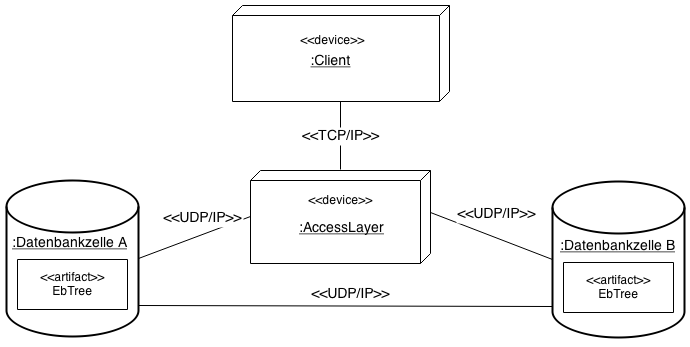
\includegraphics[width=0.8\textwidth]{bilder/uml_deployment_dia.png}
    \caption{Synchronisationsprozess}
\end{figure}
Eine weitere essentielle Komponente ist der \enquote{Accesslayer}. In diesem werden für neue Daten oder Veränderungen eindeutige \ac{ID}s erzeugt. Jedem neuen Datensatz wird eine eindeutige Nummer zugewiesen die ihn adressiert sowie eine Nummer die seine Stand wieder gibt. Neue \ac{ID}s steigen mit jeder weiterem Generierung. wird ein neuer Datensatz eingefügt oder verändert sorgt der \enquote{Accesslayer} dafür das dieser adressiert sowie an alle Datenbankzellen gesandt wird.Um auch hier Ausfallsicherheit und eine Balancierung von Last zu ermöglichen ist es möglich das mehrere \enquote{Accesslayer} parallel arbeiten. Die Koordination dieser ist eine weitere nicht triviale Aufgabe wird aber nicht weiter im Rahmen dieser Arbeit betrachtet.\\\\
\todo[inline]{Hinleitung zu Synchrobedarf da udp übertragung wegen performance} 
 Datenbanken -> in memory
Datenbanken system transparent
uml: Komponenten diagramm
Wo beschreibung der gundlegenden funktionen
grundlegende konzept mehrer Datenbanken mit gleichen Daten -> bedarf von synchronisation damit Daten konsistent bleiben

\section{Konzept der Datenbank}
\label{sec:DBConcept} 
%TODO in mermory!

Die Grundlegende Idee der Datenbank ist, nicht wie in relationalen Datenbanken Daten durch Tabellen zu gruppieren, sondern durch viele verschiedene Indexe Daten je nach benötigten Kriterien zugänglich zu machen. So kann jederzeit durch bilden von neuen Indexen auf neue Anforderungen an die Datenbank reagiert werden.\\

Neue Datensätze erhalten bei ihrer zentralen Erzeugung im \enquote{Access Layer} eine eindeutige, aufsteigende, \ac{ID}. Die Nummer ist in allen Datenbanken gleich, verändert sich nie und adressiert den Datensatz bis dieser gelöscht wird. Eine weitere Nummer, die \enquote{Change ID}, symbolisiert den Stand des Datums. Wenn das Datum angelegt wird sind Identifikationsnummer und \enquote{Change ID} identisch. Wird der Datensatz verändert wird diesem eine immer größer werdende \enquote{Change ID} zu gewiesen. Somit lässt sich leicht am Wert der \enquote{Change ID}  erkennen ob Daten verändert wurden oder sich noch ihrem Ursprungszustand befinden. Besonders praktisch ist dies beim Vergleichen von Datensätzen in unterschiedlichen Datenbanken. Durch vergleichen der \enquote{Change ID} kann so sehr schnell ermittelt werden welche von Beiden aktueller ist und der Unterschied ausgeglichen werden.\\

Für die \ac{ID}, als auch \enquote{Change ID}, wird eine eigener Index gepflegt. Hierfür wird der sich besonders gut dafür eignende, in \autoref{sec:ebTreeGrundlagen} beschriebene, \ac{EB-Baum} verwendet, da dieser auf das nach Größe sortiertem Verwalten von Ganzzahlschlüsseln optimiert ist. In die Datenbank eingefügte Datensätze werden in einem Container, dem \enquote{EbTreeDataObjekt}, gekapselt. Dieses enthält zum einen die \ac{ID}, die aktuelle \enquote{Change ID} sowie eine Referenz auf die Daten. Wird nun in die Datenbank ein Datensatz eingefügt wird dieser mit der \ac{ID} in den dazu gehörigen \enquote{ID-Baum} und mit der \enquote{Change ID} in dem \enquote{Change ID-Baum} eingefügt. Das Blatt jedes Baumes hält somit die entsprechende Nummer und den Container. Es lässt sich somit leicht auflösen welche \enquote{Change ID} mit welcher \ac{ID} und umgekehrt verbunden ist. \\\\
Beim Verändern eines Datensatzes wird die alte \enquote{Change ID} aus dem \enquote{Change ID-Baum} gelöscht und die neue \enquote{Change ID} wieder eingefügt. Da der \ac{EB-Baum} seine Schlüssel der Größe nach von links nach rechts im Baum sortiert und neu erstellte Schlüssel immer größer werden. Befinden sich neu eingefügte Elemente im \enquote{ID-Baum} sowie neu veränderte Elemente im \enquote{Change ID-Baum} ganz rechts in der Baumstruktur.\\\\
Soll ein Datum gelöscht werden werden nicht einfach die damit verknüpften Nummern und der Datensatz gelöscht. Beim Löschen muss sichergestellt werden dass das Datum aus allen Datenbanken entfernt wird da dieses sonst in der nachfolgend beschriebenen Synchronisationsprozess wieder hergestellt wird. Falls der Datensatz auf einer Seite der an Synchronisation beteiligten Datenbanken fehlt und auf der anderen Vorhanden ist lässt sich nicht feststellen ob dieses Ungleichgewicht durch ein verlorenes Einfügen oder Löschen zu Stande gekommen ist und ob das Element auf der einen Seite gelöscht oder auf der anderen wieder hergestellt werden soll. Daher werden nur die Daten des \enquote{EbTreeDataObjekt} gelöscht und eine neue \enquote{Change ID} eingefügt. Das Vollständige Löschen von \ac{ID} und \enquote{Change ID} aus beiden Bäumen sowie des \enquote{EbTreeDataObjekt} erfolgt in einem gesonderten Löschprozess der sicherstellt das diese Veränderung an jeder Datenbank vorgenommen wird.

\section{Synchronisation zwischen Datenbanken}
\label{sec:eBTreeSynchronisation}
\begin{figure}[h!]
 	\centering
    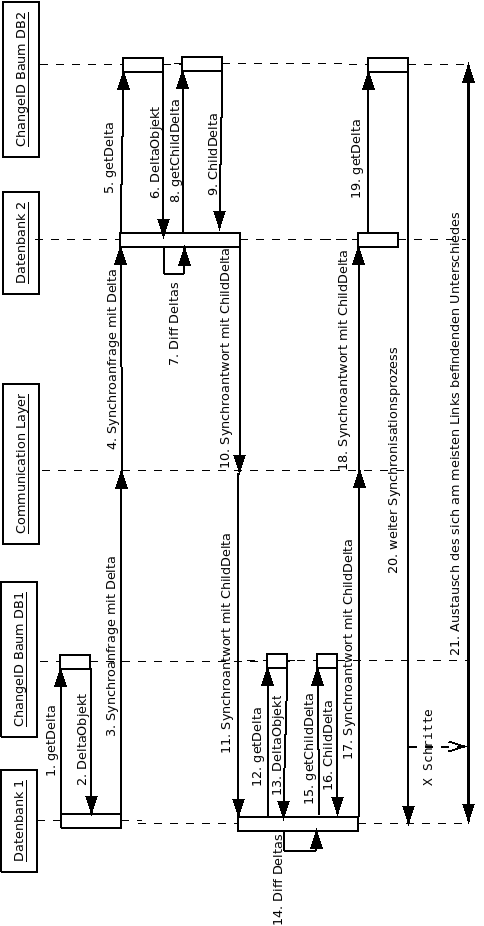
\includegraphics[width=1\textwidth]{bilder/SynchroProzess.png}
    \caption{Synchronisationsprozess}
\end{figure}
Durch ein Vergleichen der \ac{ID}s und \enquote{Change IDs} der Datensätze in den sich synchronisierenden Datenbanken kann einfach festgestellt werden welche Daten fehlen und falls diese vorhanden auf welcher Seite diese aktueller sind. Ein Vergleichen der gesamten Datenbanken jedoch, gerade wenn diese unter hoher Last stehen und sehr viele Datensätze verwalten, verbraucht viele Ressourcen. Ab einem gewissen Grad von Last durch Operationen und Masse an Daten ist dies nur schwer möglich. Ein komplettes Abgleichen nimmt in diesem Fall so viel Zeit in Anspruch dass durch neue Operationen wieder ein Ungleichgewicht zwischen den Datenbanken entstehen wird.\\\\
Daher gilt es eine Synchronisationsmethodik zu finden die zum einen in der Lage ist schnell kleine Unterschiede als auch in einer längeren Zeitspanne Datenbanken, die sich auf völlig verschiedenen Ständen befinden, auszugleichen.
Die \enquote{Change IDs}, die zum Vergleich während der Synchronisation gepflegt werden, werden in jeder Datenbank in einem \ac{EB-Baum} gehalten. Die Möglichkeit des Vergleichen von Zweigen unterhalb jedes Knotens ist daher von großem Vorteil. Um dies Möglich zu machen wird für jeden Knoten eine den Zustand seiner beiden Kindobjekte repräsentierende Nummer, die \enquote{Node Change ID}, errechnet. Dazu werden die Nummern der Kindobjekte, \enquote{Change IDs} falls das Kind ein Blatt oder \enquote{Node Change ID} falls das Kind ein Knoten ist, durch eine \enquote{binäre XOR Operation} verbunden. Während des Synchronisationsprozesses senden sich beide Seiten sogenannte \enquote{Deltas}. Es werden eine die Position des Deltaknoten beschreibenen Ganzzahl, die Bitebene des  Deltaknoten, der Bitebene des sich ber dem Deltaknoten befindenden Elternknoten, sowie die deren Zustand wieder gebenden Nummern seiner Kinder. Die übertragenen Werte bilden beschreiben das logisch zusammen hängende Dreieck aus Knoten und zwei Kindern. Daher wird es als \enquote{Delta} bezeichnet.\\
\begin{wrapfigure}{r}{0.5\textwidth}
  \begin{center}
    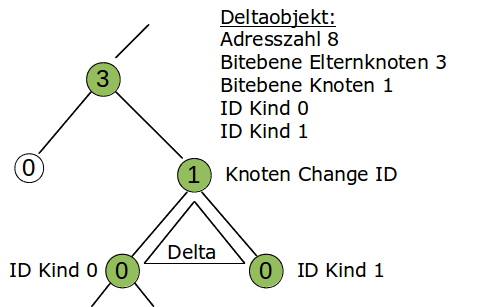
\includegraphics[width=.8\linewidth]{bilder/SynchroDelta.png}
  \end{center}
 \caption{Deltaobjekt}
\end{wrapfigure}
Durch die die Position des Deltas beschreibende Ganzzahl kann der Knoten mit dem das Delta verglichen werden soll in der anderen Datenbank gefunden werden. Bei der Lokalisierung des zu vergleichenden Knoten wird am obersten Knoten des Baumes begonnen. Je nach dem ob 0 oder 1 in der Adresszahl an der binären Stelle der Bitposition des zu durchlaufenden Knoten gesetzt ist wird das linke oder rechte Kindobjekt weiter behandelt. Dies wird solange wiederholt bis die im Delta übergebene Bitebene des Deltaelternknoten unterschritten und der sich dort befindliche zu vergleichende Knoten ermittelt ist.
Wird nach dem Vergleichen der Deltas festgestellt dass die\enquote{Node Change IDs} der linken Knoten gleich sind und die der rechten Knoten ungleich. Soll ab jetzt dieser Knoten nach rechts durchlaufen werden. Dazu wird in der binären Representation des Adresswertes an der Bitstelle die der Knoten darstellt eine 1 gesetzt und von nun an bei allen weiteren Durchläufen dieses Synchronisationsprozesses an diesem Knoten das rechte Kindobjekt behandelt.
Die Synchronisation kann von jeder Datenbank angestoßen werden. Eine Möglichkeit dies zu Koordinieren ist dass jede Datenbank zufällig in einem festgelegtem Zeitintervall zu synchronisieren beginnt. Es ist Möglich das sich die Datenbank während des Synchronisationsprozess verändert. Die Synchronisation besteht aus zwei Phasen. 
\subsection{Synchronisation Phase 1} 
In der Ersten Phase gilt es den Unterschied zu finden der sich in beiden Bäumen am weitesten links befindet und somit die älteste Unterschied zwischen den Datenbanken darstellt. Da im laufenden Betrieb auf der rechten Seite des Baumes viele Veränderung statt findet soll immer der Unterschied der davon am weitesten Entfernt liegt zu erst behoben werden. Daten die sich oft Verändern sind sehr weit rechts im Baum zu finden und da somit besteht die Chance dass sich mögliche verlorene Veränderungen bei einer erneuten Veränderung selbst ausgleichen.
Die mit der Synchronisation beginnende Datenbank sendet ein Delta des höchsten Knoten gekapselt in einer Synchronisationsanfrage an die andere Datenbank. Diese lokalisiert den Knoten mit dem das Delta abgeglichen werden soll und vergleicht die Nummer des linken Kindobjektes des erhaltenen Delta mit dem linken Kindobjekt des eigenen Knotens. Sind diese gleich werden die rechten Kindobjekte verglichen. Wird dabei kein Unterschied erkannt sind die Datenbanken synchron und der Synchronisationsvorgang ist abgeschlossen. Falls aber ein Unterschied lokalisiert werden kann wird mit einem Delta bestehend aus dem sich unterscheidenden Kindobjektes geantwortet. Die sich synchronisierenden Datenbanken spielen mit dem Senden der Deltas eine Art von \enquote{Ping-Pong} bis der am weiten links liegende Unterschied gefunden ist.\\\\
Beim Abgleichen der Deltas kommt es zu unterschiedlichen Vergleichsfällen die vom Synchronisationsalgorithmus separat behandelt werden müssen:

\subsubsection{Unterschied Links/Rechts}
\label{sec:SynchroDiffLeftOrRight}
Die Knotenstruktur in den \enquote{Change ID-Bäumen} beider Datenbanken ist bis zum ersten Unterschied identisch. Der Synchronisationsalgorithmus läuft Delta für Delta die Bäume entlang und navigiert dabei je nach gefundenem Unterschied nach Links oder Rechts bis ein Blatt gefunden wird. Es besteht aber nun die Möglichkeit das an der Stelle wo das Blatt gefunden wurde sich im anderen Baum ein Zweig befindet in dem das Blatt bereits vorhanden ist, \autoref{fig:Case1TreeB,B*}. Beim Vergleichen der \enquote{Change IDs} wird ein Unterschied festgestellt doch dieser befindet sich im Unterzweig der anderen Datenbank. Bevor dieser aber lokalisiert werden kann wird in der Datenbank ohne den Unterzweig bereits dass Blatt gefunden. Daher wird sobald ein Blatt gefunden wird dessen ID der anderen Seite mitgeteilt und dort geprüft ob diese bereits vorhanden ist. Falls das Blatt noch nicht vorhanden ist werden nun die kompletten Daten des Blattes angefordert und eingefügt.\begin{wrapfigure}{r}{0.5\textwidth}
  \begin{center}
    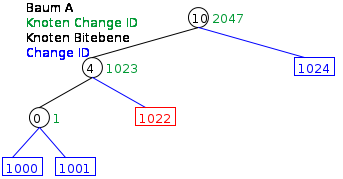
\includegraphics[width=0.9\linewidth]{bilder/Case1TreeA.png}
  \end{center}
 \caption{Baum A}
 \label{fig:Case1TreeA}
\end{wrapfigure} Ist das Blatt aber bereits im Baum wird an die Position des Unterzweig gelaufen und dort das linkeste Blatt betrachtet. Ist dieses nicht das gefundene Blatt wurde der sich am weitesten Links befindende Unterschied gefunden und der Datensatz zum Einfügen an die andere Datenbank gesandt. Ist das linkeste Blatt aber das Gefundene ist der linkeste Unterschied der nächste rechte Nachbar und kann ausgetauscht werden.
\begin{figure}[h!]
  \begin{center}
    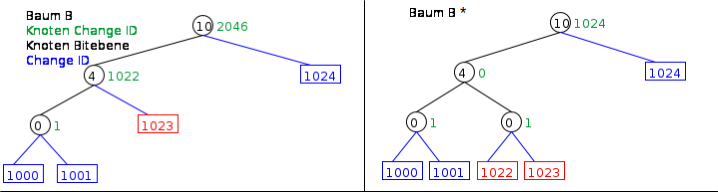
\includegraphics[width=0.9\linewidth]{bilder/Case B Baeume.png}
  \end{center}
 \caption{Baum B, B*}
  \label{fig:Case1TreeB,B*}
\end{figure}

\subsubsection{Behandeln von verschieden vielen Bitebenen} 

Je nach dem wie groß sich die Bäume unterscheiden so verschieden ist auch die Strukturen an Knoten. Das führt so folgender Problematik. Der älteste gesuchte Unterschied liegt links im Baum doch Fehlen ebenfalls andere, neuere Werte und somit auch die Knoten die mit ihnen erzeugt werden. Ein einfaches \enquote{Delta Ping-Pong} Knoten für Knoten und dabei Bitebene für Bitebene ist daher nicht möglich. Auch ist davon Auszugehen das es Möglich ist das auf beiden Seiten Bitebenen fehlen. Dies führt zu einer Vielzahl an Möglichkeiten in denen sich bei Seiten unterscheiden können. Um die Lücken an Knoten zu erkennen und zu behandeln ist in den Deltaobjekten die Bitebene des Deltaknoten sowie die Bitebene des obehalb liegenden Elternknoten enthalten.\\\\
Zu beginn eines Synchronisationsschrittes wird im Baum der Knoten ermittelt der sich unterhalb der Bitebene des Elternknoten des erhaltenen Deltas befindet. Dazu wird der Baum mit der Adresszahl solange durchlaufen bis die Bitebene des betrachteten Knoten die Bitebene des Elternknoten des erhaltenen Deltas unterschreitet. Nun wird geprüft ob die Bitebene des gefundenen Knoten gleich der  Bitebene des erhaltenen Deltaknotens ist. Ist dies der Fall wird mit der im oberen \autoref{sec:SynchroDiffLeftOrRight} beschriebenen Prozedur verfahren. Unterscheiden sich die Bitebenen führt dies zu zwei Möglichkeiten. 
\begin{figure}[h!]
  \begin{center}
    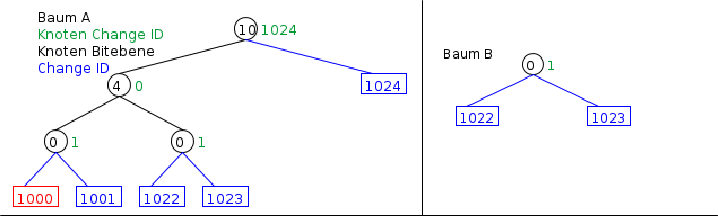
\includegraphics[width=0.9\linewidth]{bilder/case 2 a* B**.png}
  \end{center}
 \caption{Bäume mit verschieden vielen Bitebenen}
\end{figure}\\
Die Bitebene des gefundenen Knotens ist kleiner als die des Deltaknoten. Zwischen den beiden Knoten befindet sich Loch in dem sich noch noch nicht synchronisierte Blätter und dazu gehörige Knoten befinden. Doch diese sollen vom Algorithmus erst später repariert werden da diese neuer und zu erst der ältesten Unterschied behoben werden soll. Daher gilt es das Loch zu überspringen. Dazu sendet die Seite mit dem tieferen Knoten ein spezielles Delta zurück welches das nächste linke Delta unterhalb des erhaltenen Delta anfordert. Dies wird solange wiederholt bis auf beiden Seiten die selbe Bitebene erreicht ist oder falls die kleine Bitebene im anderen Baum nicht vorhanden ein Blatt gefunden wird. Ist auf beiden Seiten die gleiche Bitebene erreicht können die Kinderobjekte wie im oberen \autoref{sec:SynchroDiffLeftOrRight} beschrieben verglichen werden.
Falls aber die Bitebene des gefundenen Knoten größer ist als die des Deltaknotens wird ein Delta aus dem gefundenen Knoten gebildet und zurück gesandt. Damit werden einfach die Seiten getauscht und der gerade beschriebene Fall tritt ein. Diese Methodik wird ebenfalls genutzt um mit Synchronisation zu beginnen. Einer der Datenbanken wird ein manipuliertes Deltaobjekt gesandt. Dieses trägt als Absender die andere Datenbank. Die Werte der Bitebenen von Deltaknoten und Elternknoten sind negativ. Somit wird zuerst der oberste Knoten lokalisiert. Da dessen Ebenenbit positiv ist und somit größer als der erhaltene negative Deltawert wird der oberste Knoten als Delta an die andere Datenbank gesandt und ein Synchronisationsschritt beginnt. \\\\
\begin{figure}[h!]
  \begin{center}
    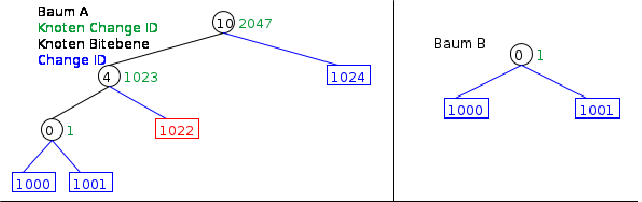
\includegraphics[width=0.9\linewidth]{bilder/case 2 A B1.png}
  \end{center}
 \caption{Bäume mit verschieden vielen Bitebenen}
\end{figure}
Ein weiterer Sonderfall tritt ein wenn der Knoten und seine unter im liegenden Kinder des Baumes mit fehlenden Knoten im anderen Baum bereits vollständig enthalten ist und sich der gesuchte Unterschied oberhalb davon befindet. Während des angleichen der Bitebenen werden keine \enquote{Change IDs} verglichen. Erst wenn auf beiden Seiten die selbe Bitebene erreicht ist wird wieder nach Unterschieden geprüft und in diesem Fall  Links und Rechts keine Unterschiede gefunden werden was die Bäume als synchron erscheinen lassen wird. Daher muss immer beim Überspringen des Bitebenenlochs bevor das nächst tiefere Delta angefordert wird überprüft werden ob dieses bereits die selbe \enquote{Change ID}  hat wie der Knoten. Ist dies der Fall liegt der gesuchter Unterschied ganz links im rechten Kindobjektzweig oder ist das Kindobjekt selbst.

\todo[inline]{Special case node nicht im anderen baum}


\subsection{Synchronisation Phase 2}
Nach Ablauf der ersten Synchronisationsphase ist die sich, in den \enquote{Change-ID Bäumen}, am weitesten Links befindende, unterscheidende \enquote{Change-ID} gefunden. Nun sendet die Datenbank in der sich diese befindet das gesamte \enquote{EbTreeDataObjekt} auf welches die \enquote{Change-ID} referenziert an die andere Datenbank in der die \enquote{Change-ID} nicht vorhanden ist. Durch die im \enquote{EbTreeDataObjekt} enthaltene \ac{ID} kann nun im  \enquote{ID-Baum} geprüft werden ob diese enthalten ist. Falls dies nicht der Fall ist die komplette Einfügeoperation des Datensatzes verloren gegangen und dieser muss nun nachträglich in beide Bäume eingefügt werden. Ist es Möglich die \ac{ID} zu lokalisieren ist dass \enquote{EbTreeDataObjekt} bereits in beiden Datenbanken vorhanden aber auf einem unterschiedlichem Stand. Nun gilt es durch einen Vergleich der beiden \enquote{Change-IDs} heraus zu finden auf welcher Seite der Datensatz aktueller ist und dies auszugleichen. Ist die erhaltene \enquote{Change-ID} größer als die Eigene wird der eigene Datensatz aktualisiert. Ist aber die erhaltene \enquote{Change-ID} kleiner kann der eigene Datensatz als Update an die andere Datenbank gesandt werden. Der Synchronisationsschritt ist abgeschlossen. Egal ob eine veraltete oder aktuelle  \enquote{Change-ID} gefunden wird jeder Synchronisationsschritt führt zum Ausgleich eines Unterschiedes.
	
\section{Architektur des Prototypen}
\begin{figure}[h!]
  \begin{center}
    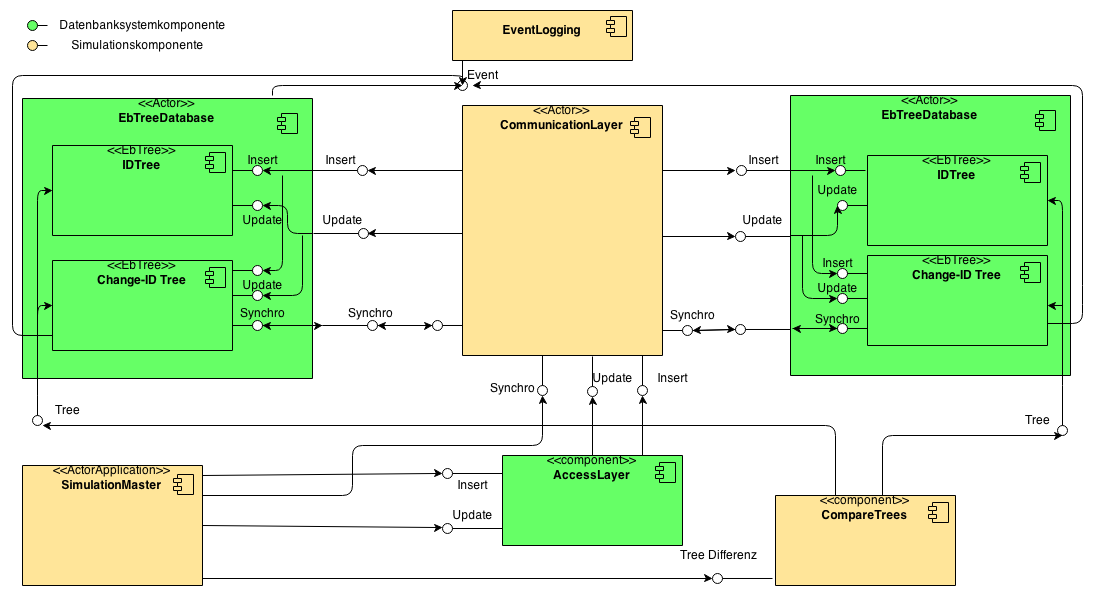
\includegraphics[width=1.0\linewidth]{bilder/prototyp_component_diagram.png}
  \end{center}
 \caption{UML Komponentendiagramm des Prototypen}
\end{figure}
\todo[inline]{ turn picture}
Der in dieser Arbeit erstellte Prototyp besteht grundlegend aus zwei Teilen. Er besteht zum einen aus den Komponenten des in \autoref{sec:DBConcept} beschriebenen Datenbankkonzeptes und der in \autoref{sec:eBTreeSynchronisation} erklärten Synchronisation zwischen zwei Instanzen der Datenbank. Zum anderen einer Simulationsumgebung mit welcher die Funktionalität des Datenbanksystem getestet werden kann. Die Synchronisation zwischen den einzelnen Datenbankinstanzen kann hier ebenfalls getestet und analysiert werden. Durch verschiedene Initialisierungen des Datenbanksystem und dem erzeugen von Last  können verschiedene Szenarios erzeugt und die Leistung des Systems bewertet werden. \\

Die Applikation ist zum Teil als Actorsystem umgesetzt. So wird jede Datenbank, als auch der \enquote{CommunicationLayer}, welcher als Bindeglied zwischen den Komponenten fungiert, durch einen Aktor repräsentiert.
Das Senden von Actornachrichten ähnelt dem Senden von IP-Paketen zwischen zwei Datenbanken an verschiedenen Standorten. Wann welche Nachricht und in welcher Reihenfolge bei welcher Datenbank ankommt ist nicht vorhersehbar. Verlust oder Verspätung von Paketen und die daraus resultierende Ungleichheit der Datenbanken lassen sich so gut simulieren.

 Zwischen den Datenbankaktoren befindet sich, als Teil der Simulationsumgebung, ein Kommunikationsebene. In dieser können  Verlust und Verspätung von Paketen gesteuert werden.


\subsection{Datenbankkomponenten}
Der Prototyp setzt einen Teil der in \autoref{sec:DBSystemConcept} beschriebenen Komponenten um. Die Generierung von \ac{ID}s die neue Daten zu adressieren und den Stand von Aktualisierungen abbilden werden in einer Basisimplementierung des \enquote{Accesslayer} generiert. Diese werden mit den Daten in einem \enquote{EbTreeDataObjekt} gekapselt und alle Datenbankzellen gesandt. Jeden Datenbankzelle wird durch einen Actor repräsentiert und kann Nachrichten mit neuen Daten, Änderungen oder Synchronisationsanfragen erhalten und senden. Im Rahmen dieser Arbeit werden zwei Datenbankzellen verwendet und Operationen wie Einfügen, Aktualisieren oder Löschen sowie die Synchronisation zwischen beiden getestet. Die Datensätze werden in einer Erweiterung des klassischen \ac{EB-Baum} gehalten.

\subsection{Simulationskomponenten}	
Die Komponenten der Simulationsumgebung setzen auf den Datenbankkomponenten auf. Zwischen den zwei Datenbankzellen und dem \enquote{Accesslayer} wird der \enquote{CommunicationLayer} zwischen geschoben. Der \enquote{CommunicationLayer} ist wie die zwei Datenbankzellen ein Actor. Durch ihn läuft die gesamte Kommunikation aller Komponenten. Werden neue Daten Eingefügt oder Aktualisiert werden diese vom \enquote{Accesslayer} an den \enquote{CommunicationLayer} übergeben und an die zwei Datenbanken weiter verteilt. Auch die Synchronisation zwischen den beiden Zellen läuft durch \enquote{CommunicationLayer}. Die Daten die im Datenbankystem gekapselt in \enquote{EbTreeDataObjekten} oder \enquote{Deltaobjekten} versandt werden werden als Nachrichten zwischen den Actoren versandt. Jede Nachricht passiert \enquote{CommunicationLayer} und kann somit in diesem beeinflusst werden. So kann ein Prozentwert eingestellt werden mit dem Pakete verloren gehen um das Senden von UDP-Paketen zu simulieren. Auch die Verzögerung von Paketen kann hier simuliert werden. Neue Datensätze oder Aktualisierungen alter Daten werden in einer \enquote{Queue} abgelegt. Soll ein Paket verzögert werden wird es einfach je nach dem wie stark die Verzögerung sein soll weiter hinten eingereiht und somit später versandt.Durch Verlust und Verzögerung werden die Datenbestände in beiden Datenbanken verschieden. Je nach dem wie hoch Verzögerung und Verlust im \enquote{CommunicationLayer} eingestellt sind können in anderen Teilen der Simulationsumgebung die Auswirkungen auf das gesamte System und die Synchronisation ermittelt werden.\\\\
Start Punkt der Simulationsumgebung als auch des gesamten Prototypen ist der \enquote{SimulationMaster}. In dieser Komponente wird beim Start des Prototypen das Actorsystem initialisiert. Die beiden Datenbankzellen, \enquote{Accesslayer} und \enquote{CommunicationLayer} werden instanziiert, deren Referenzen unter den Komponenten ausgetauscht und das gesamte Datenbanksystem sowie die Simulationsumgebung selbst initialisiert. Aufgabe des \enquote{SimulationMaster} ist es zum einen das System zu initialisieren und zu starten und anschließend eine Reihe verschiedene Simulationen zu ermöglichen. Während der Simulation werden Daten ausgewertet und diese in einem einer CSV-Datei gespeichert. Welche Simulation ausgeführt werden soll kann vom Nutzer in einem einfachen \enquote{Kommandozeileninterface} ausgewählt werden. Je nach Simulation wird nun das Datenbanksystem mit Daten initialisiert und mit der Simulation begonnen. Während der Simulation kann der Inhalt der einzelnen Zellen verändert werden um Last auf das Datenbanksystem zu simulieren. Der \enquote{SimulationMaster} generiert dazu neue Daten oder Änderungen und sendet diese, via dem \enquote{AccessLayer}, an den \enquote{CommunicationLayer}. Dort wird nun entschieden ob das Paket Verloren geht oder Verspätet wird und anschließend dieses in der \enquote{Queue} abgelegt. Der \enquote{SimulationMaster} sendet in gewissen Intervallen ein \enquote{Clocksignal} welches dafür sorgt dass das die Pakete im ersten Feld der \enquote{Queue} versandt werden. Je nach dem wie hoch der Verlust oder die Verspätung von Paketen eingestellt ist ergibt sich ein Unterschied zwischen den Zellen der mit der Synchronisation ausgeglichen werden soll. Die Synchronisation der Datenbankzellen wird ebenfalls im \enquote{SimulationMaster} gestartet. Dazu wird an den \enquote{CommunicationLayer} eine Nachricht gesandt das mit der Synchronisation eines Unterschiedes begonnen werden soll. In der Nachricht ist enthalten welche Datenbank mit der Synchronisation beginnt. Der \enquote{SimulationMaster} wartet nun bis die Synchronisation eines Unterschiedes abgeschlossen ist und fährt mit der Simulation fort.\\\\
Um den Erfolg der Synchronisation und das Entstehen von Unterschieden bestimmen zu können existiert die Komponente \enquote{TreeCompare}, die den Unterschied beider Datenbanken bestimmt werden kann. Um den Unterschied zu bestimmen werden die \enquote{ID-Bäume} und \enquote{Change ID-Bäume} beider Datenbanken Blatt für Blatt verglichen und gezählt um wie viele Elemente sich Unterscheiden. Beim Vergleichen der \enquote{ID-Bäume} kann festgestellt werden um wie viele Einfügeoperationen und beim Vergleichen der \enquote{Change ID-Bäume} wie viele Aktualisieren sich beide Datenbanken unterscheiden.

%TODO eventlogging
%---------------------------------------------------------------------------------------------------------------------------------------------------
\chapter{Implementierung}
\todo[inline]{Realisierung/Umsetzung, Beschreibung der Implementierung, nicht des Programmcodes}
		\begin{enumerate}[1.]
			\item Umsetzung der Systemarchitektur
			\item Beschreibung und Besonderheiten der Implementierung
		\end{enumerate}

\section{EBTree} % teil gurndlage teil implementation
Die im Rahmen dieser Arbeit erstellte Scalaimplementierung des \enquote{Elastischen Binär Baums} orientiert sich zum einen an dem in Grundlagen~\ref{sec:ebTreeGrundlagen} beschriebenen Entwurf von Willy Tarreau\autocite{Tarreau}, als auch auf einer mehr spezifischen Basisumsetzung der Spinning Wheel GmbH.\\
In dieser wird bereits die enge Koppelung von Knoten und Blättern, der ursprünglichen C Implementation, aufgebrochen.\unsure{SPW c umsetzung mit blatt+node pointerns?}Die zuvor in \enquote{C structs} aufgebauten Knoten und Blätter wurden durch Java Klassen ersetzt und ihre gemeinsame Eigenschaften in einem Interface definiert. Basisfunktionen des Baumes wie einfügen, löschen und durchlaufen des Baumes waren hier ebenfalls vorhanden und wurden als Teil der Arbeit in Scala neu umgesetzt.\\\\
Eine besondere Anforderung an den Baum ist das die sortiert, verwalteten Schlüssel einzigartig sind und ein Einfügen von Duplikaten verhindert wird. Da das Verwalten von Duplikaten an sich möglich ist aber für das Funktionieren des Baumes nicht zwingend nötig wird ein einfügen dieser, bei der folgend beschrieben Umsetzung, vermieden. \\
\subsection{Grundlegender Aufbau}
Der Baum selbst ist einer eigenen, generischen Klasse umgesetzt. Diese besteht aus den Funktionalitäten des Baumes, zwei \enquote{Case-Klassen}, repräsentativ für Knoten und Blätter, sowie einem \enquote{Trait} der deren gemeinsame Eigenschaften beschreibt. Der generische Typ der Klasse wird bei deren Instanziierung übergeben und legt den Datentyp der in den Blättern gespeicherten Daten fest. Somit kann der Baum jeder Art von Daten halten ohne verändert werden zu müssen.\\

Der \enquote{Trait} Child beschreibt was dass \enquote{Kind} eines Knoten können muss. Ganz gleich ob es sich hier um ein Blatt oder einen weiteren, einen neuen Zweig öffnenden, Knoten handelt. Festgelegt ist das ein jedes \enquote{Kindobjekt} eine Referenz auf ein \enquote{Elternobekt} haben muss und eine Methode die die eindeutig identifizierbare ID des Objektes zurück gibt. Die ID ist bei Blättern der Schlüssel mit dem das Blatt eingefügt wird und bei Knoten die \enquote{Node Change ID} welche zum vergleichen von Baumzweigen anderer Datenbanken bei der Synchronisation verwendet wird.\\

Durch den Einsatz von \enquote{Case-Klassen} kann durch \enquote{Pattern Matching} beim durchlaufen des Baumes sehr einfach geprüft werden welcher Klasse Kindelemente angehören und diese verarbeitet werden.\\

Die Aufgabe des Blatt \enquote{Case Klasse} ist sehr einfach. Sie hält die Referenz auf einen übergeben Datensatz und ist durch einen eindeutige Schlüssel identifizierbar. Knoten hingegen verfügen über mehr Logik. So kann dieser die in seiner Wurzel gespeicherten Kindobjekte, weitere Zweige oder Blätter, zurück geben oder neue anfügen. Durch sein Ebenenbit weiß ein Knoten auf welcher binären Ebene des Baumes er steht und kann in dem, bei einer Abfrage- oder Einfügeoperation, übergebenen Schlüssel an der entsprechenden Stelle nachschauen und seinen linkes oder rechtes Kindobjekt verarbeiten.

\begin{listing}[H]
	\begin{minted}[mathescape,
	               numbersep=5pt,
	               frame=lines,
	               framesep=1mm]{scala}
case class Node[T](myBit: Int) extends Child[T] {
    var myZero:				Child[T]  = _
    var myOne:				Child[T]  = _
    var nodeChangeID:	Long    	= _

    def bitOne(uid: Long): Boolean = ((uid & (1L << myBit)) != 0) && (myBit < 64)

    def getChild(uid: Long): Child[T] = bitOne(uid) match {
      case true => myOne;
      case false => myZero
    }
    def setChild(uid: Long, child: Child[T]) = {
      bitOne(uid) match {
        case true => myOne = child
        case false => myZero = child
      }
      child.myParent = this
    }
    override def getID(): Long = nodeStateID
  }	
	\end{minted}
	\caption{Umsetzung eines Knoten des \ac{EB-Baum}}
	\label{lst:Knoten EB-Baum}
\end{listing}

-> klassen bild\\
\subsection{Funktionalität des Baumes}
\subsubsection{Finden von Schlüsseln}
Die Suche eines Schlüssel ist durch schlanke rekursive Funktion gelöst. Der zu suchende Schlüssel gibt einen Art binären Weg vor. So beginnt die Funktion am ersten Knoten des Baumes. Diesem wird der zu suchende Schlüssel übergeben. Der Knoten weiß durch sein Ebenenbit welche Stelle er in binären Repräsentation des Schlüssels ein nimmt. Je nach dem ob das Bit an dieser Stelle 0 oder 1 ist gibt er sein linkes oder rechtes Kindobjekt zurück. Nun kann via \enquote{Pattern Matching} unterschieden werden ob es sich bei diesem um einen weiteren Knoten handelt oder ein Blatt handelt. Ist das gefundene Objekt ein Blatt wird die Rekursion abgebrochen und das Blatt zurück gegeben. Falls ein Blatt mit dem gesuchten Schlüssel im Baum vorhanden ist wird dieses oder das Blatt mit am dem nächst kleinerem Schlüssel beim durch laufen des Rekursion gefunden. Falls das gefundene Objekt aber ein, einen weiterer einen neuen Zweig öffnenden, Knoten ist wird mit diesem die rekursive Funktion erneut aufgerufen bis ein Blatt gefunden wird.
\subsubsection{Einfügen eines neuen Datensatzes}
Beim einfügen eines neuen Blatt wird zunächst der Baum nach seinem Schlüssel durchsucht. Falls der Schlüssel bereits vorhanden ist wird der neuen Datensatz im gefundenen Blatt eingefügt und der Alte zurück gegeben. So wird verhindert das Duplikate eingefügt werden können. Falls der Schlüssel nicht vorhanden ist und sich bereits Blätter im Baum befinden wird zu nächst das Blatt gefunden dessen Schlüssel die ähnlichste binäre Repräsentation besitzt. Nun werden die Schlüssel des neuen und des gefundenem Blattes durch eine binäre Oder-Operation verknüpft und  die Bitstelle des höchsten Bitunterschiedes ermittelt. Diese wird das neue Ebenenbit des Knoten der mit dem Blatt eingefügt wird. Nun muss die passende Ebene im bereits durch die Suche ermittelten Zweiges gefunden werden. Dazu wird das Ebenenbit des Elternknoten des gefundenen Blattes mit dem neue bestimmten Ebenenbit verglichen ist das Neue kleiner wurde die richtige Ebene gefunden andernfalls wird der Zweig Knoten für Knoten nach oben durchlaufen bis die passende Stelle gefunden ist. An dieser kann der neue Knoten samt Blatt eingehängt werden. Das Durchlaufen dieses Algorithmus stellt sicher das ein neuer Schlüssel stets an der richtigen Stelle eingefügt wird und der Baum aufsteigend von links nach rechts sortiert ist.

\subsubsection{Erzeugen von Knoten Status IDs}
Das vergleichen von Blättern ist durch deren einzigartige, aufsteigenden Schlüssel einfach um zu setzen. Bei dem, in dieser Arbeit umgesetzten, Synchronisationansatz, ~\autoref{sec:eBTreeSynchronisation}, muss es aber möglich sein ganze Zweige unterhalb eines Knotens zu vergleichen. Daher besitzt der Baum eine Funktion die es ermöglicht für jeden Knoten eine Nummer, die \enquote{Knoten Status ID}, zu erzeugen die den Zustand seiner beiden Kinder repräsentiert.\\

Wird ein Blatt angefügt oder gelöscht werden die \enquote{Knoten Status ID} rekursiv nach oben bis zur Wurzel generiert. Hierfür werden die IDs seiner Kindobjekte einfach durch eine binäre Oder-Operation verknüpft. Ist das Kindobjekt ein Blatt wird als ID der Schlüssel verwendet. Ist das Objekt ein Knoten seine bereits berechnete \enquote{Knoten Status ID}. 

\subsubsection{Methoden zur Synchronisation}

\subsubsection{Durchlaufen des Baumes}

\subsubsection{Weitere Funktionen des Baumes}
-> aendern eines elementes 
-> entfernen eines elementes


-> immer sortiert , Elemente werden nach einem Wert hier cID und uID eingefügt und automatisch nach rechts aufsteigend sortiert
binaerlogik beschreiben




	\section{TreeActor}
-> haelt 2 bäume für uID udn cID

\section{Acceslayer}

\section{Vergleichen von Bäumen}

%---------------------------------------------------------------------------------------------------------------------------------------------------
\chapter{Test}
\todo[inline]{Testarten, Testkriterien, Testumgebung, Testergebnisse}
		\begin{enumerate}[1.]
			\item Testkriterien und Szenarien
			\item Demonstration der Funktionalität
			\item Auswertung der Ergebnisse
		\end{enumerate}
		
Test run with different start data -> check which case gets more often
check id length xor problem
sync ops frequency		
%---------------------------------------------------------------------------------------------------------------------------------------------------		
\chapter{Fazit und Ausblick alias Ergebnis}
\todo[inline]{Zusammenfassung, Bewertung der Ergebnisse, Vergleich mit der Zielstellung, Ausblick}

- spannende basisumsetzung mit viel potenzial da erste hindernisse ueberwunden viel moeglichkeiten der optimierung\\
- komplexitaets berechnung vs annahme des brutforcealgo -> spannend waeren "delta vs brutforce perfomance test"\\
- optimize Synchro bigger deltas, abkuerzungen optimierung\\

die anzahl der synchronisationen selbst regulierender algorithmus -> check ob er im Baum vorwaerts nach rechts kommt und beschleinigung\\
\newpage
\listoftodos[Notes]

\newpage
\printbibheading
\printbibliography[type=book,heading=subbibliography,title={Buch Quellen}]
\printbibliography[nottype=book,heading=subbibliography,title={Andere Quellen}]
%\printbibliography[keyword=major,heading=subbibliography,title={Major Sources}] -> add keywords via jabref in the bibFile
%\printbibliography[keyword=minor,heading=subbibliography,title={Minor Sources}]

\chapter{Verzeichnisse}
\todo[inline]{Glossar, Abkürzungen, Abbildungen, Tabellen}

\chapter{Anhang}
\todo[inline]{technische Dokumentation, Benutzerhandbuch, Installationsbeschreibung}

\newpage

\hfil\\\\\\

\begin{LARGE}
\textbf{Eigenständigkeitserklärung}\\\\
\end{LARGE} 
Hiermit versichere ich, dass ich die vorliegende Bachelorarbeit selbstständig und nur
unter Verwendung der angegebenen Quellen und Hilfsmittel verfasst habe. Die Arbeit
wurde bisher in gleicher oder ähnlicher Form keiner anderen Prüfungsbehörde vorgelegt.\\\\\\

\parbox{4cm}{\centering Berlin, 04.02.2014\hrule
\strut \centering\footnotesize Ort, Datum} \hfill\parbox{4cm}{\hrule
\strut \centering\footnotesize Unterschrift}

\end{document}
%EINFACH MACHEN!